\chapter{Baadal Sandbox Setup Usage}


Following are the steps to start with sandbox server we established:-

\begin{enumerate}
    \item Login to server used for baadal sandbox setup
    
\begin{minipage}{\linewidth}
\centering
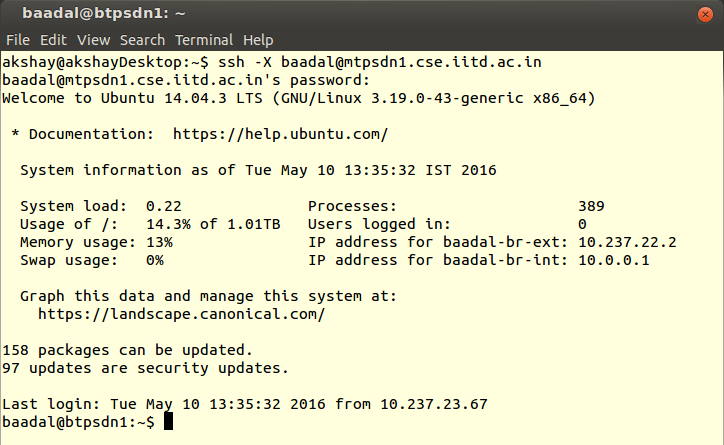
\includegraphics[width=0.9\textwidth]{first_login}
\captionof{figure}{Login to the baadal sandbox server}
\end{minipage}

\newpage
\item For status of VMs running in sandbox we can use \textit{sudo virsh list --all}
\begin{figure}[h]
\caption{Different VMs running in the sandbox}
\centering
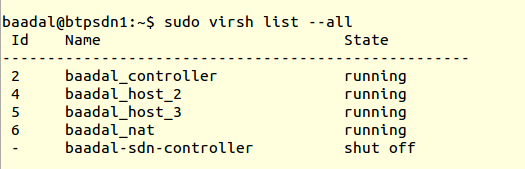
\includegraphics[width=0.9\textwidth]{Status_VMs}
\end{figure}


\item Using \textit{ifconfig} we can see the network configuration for the server.
\begin{figure}[h]
\caption{Output of ifconfig command on sandbox server}
\centering
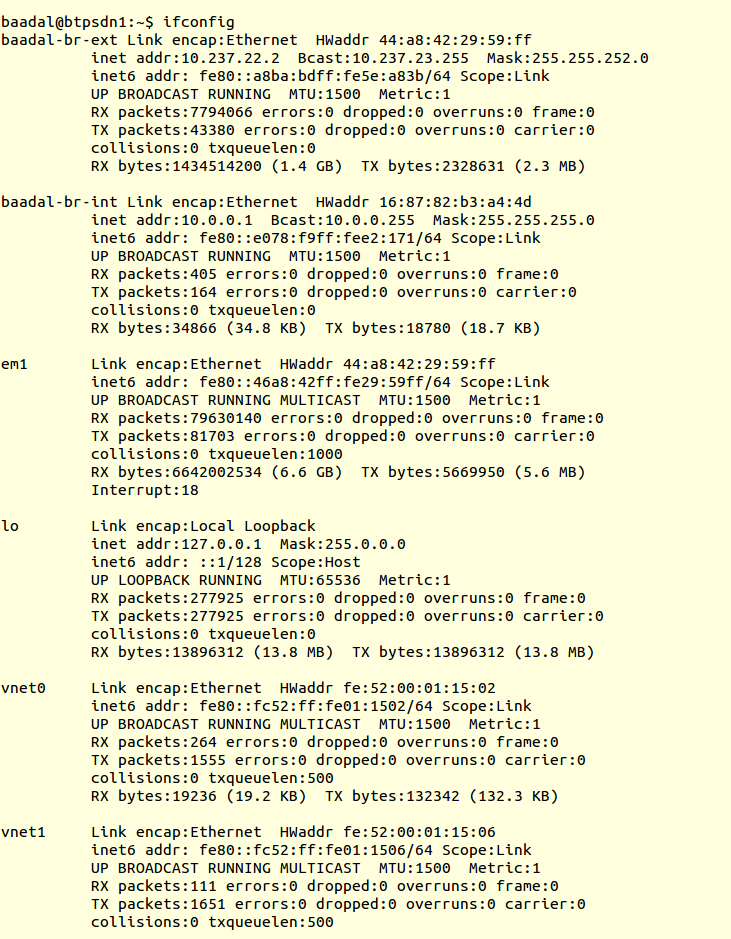
\includegraphics[height=10cm, width=0.9\textwidth]{ifconfig_server}
\end{figure}

\newpage
\item login inside the controller

\begin{figure}[h]
\caption{Login in the baadal controller}
\centering
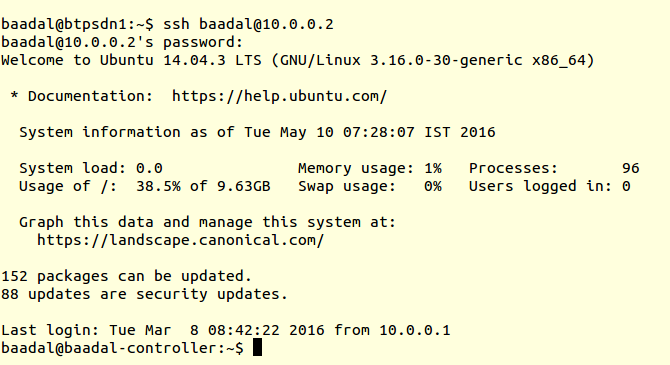
\includegraphics[height = 5cm, width=0.9\textwidth]{login_controller}
\end{figure}


\begin{figure}[h]
\caption{ifconfig showing 255 fake bridges inside the controller}
\centering
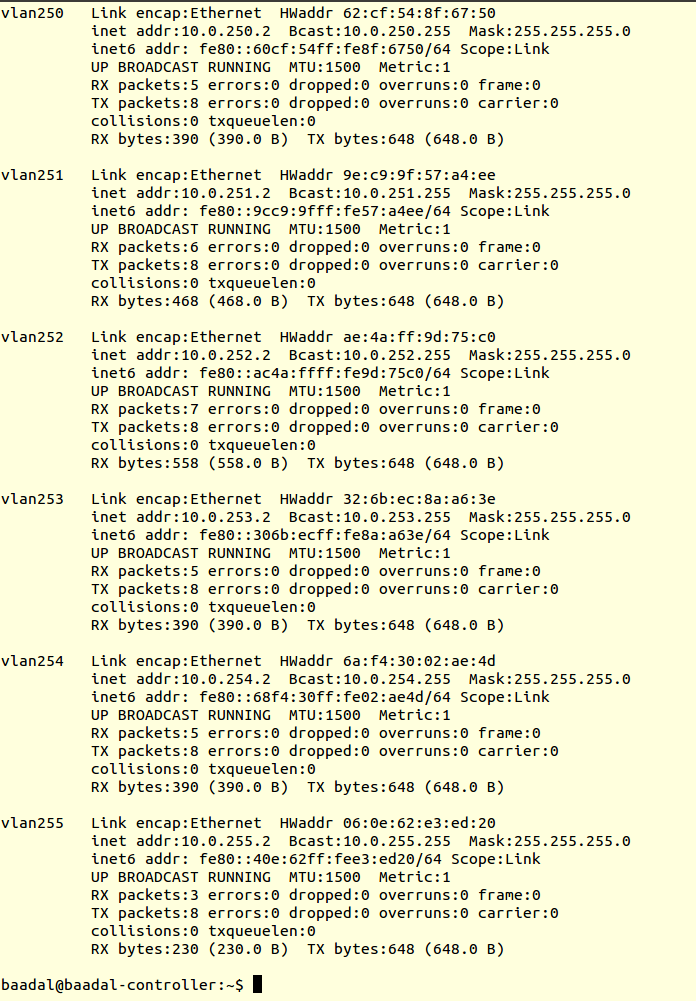
\includegraphics[height=9cm, width=0.9\textwidth]{ifconfig_controller}
\end{figure}

\begin{figure}
\caption{Web2py Processes Running inside controller}
\centering
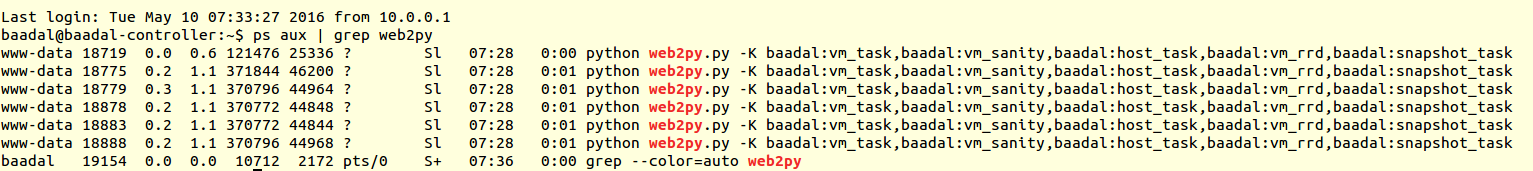
\includegraphics[width=0.9\textwidth]{web2py_processes_controller}
\end{figure}

\newpage
\item Login inside the nat is shown as

\begin{figure}[h]
\caption{Login inside the nat}
\centering
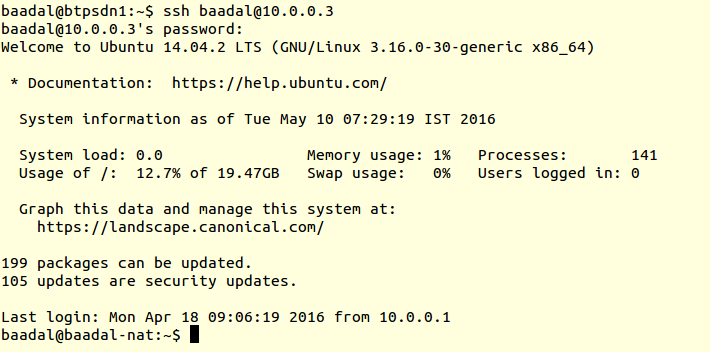
\includegraphics[width=0.9\textwidth]{login_nat}
\end{figure}


\begin{minipage}{\linewidth}
\centering
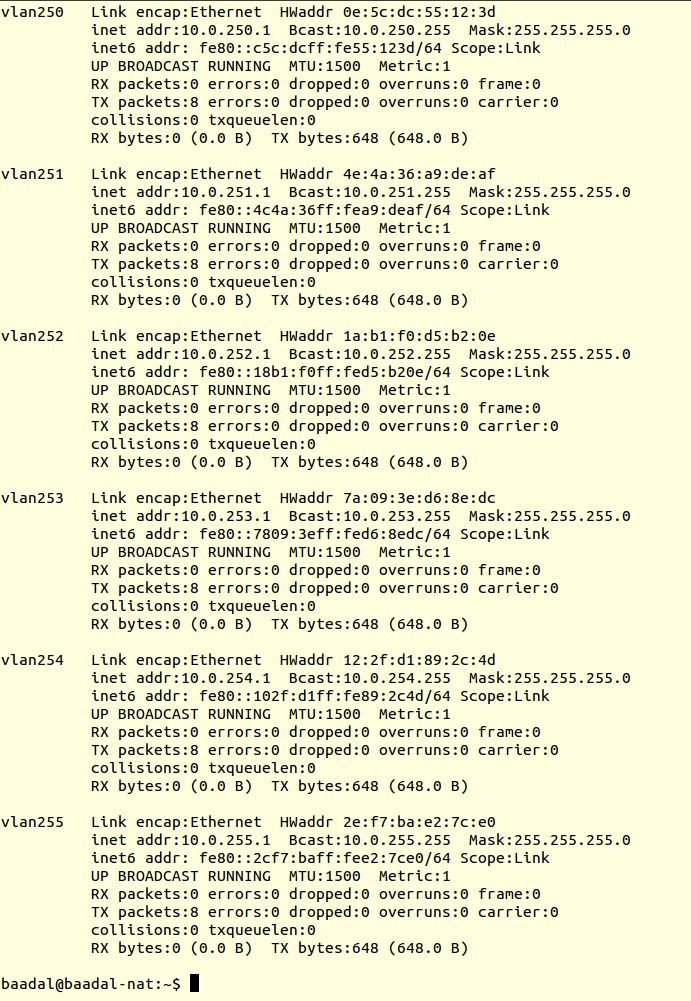
\includegraphics[width=0.9\textwidth]{ifconfig_nat}
\captionof{figure}{ifconfig showing 255 fake bridges inside the NAT}
\end{minipage}

\item Login inside host

\begin{minipage}{\linewidth}
\centering
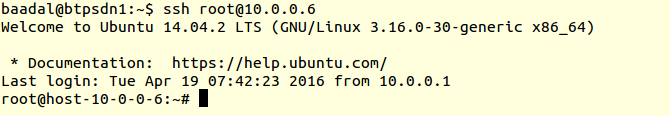
\includegraphics[width=0.9\textwidth]{login_host_6}
\captionof{figure}{Login inside host 10.0.0.6}
\end{minipage}


\begin{minipage}{\linewidth}

\centering
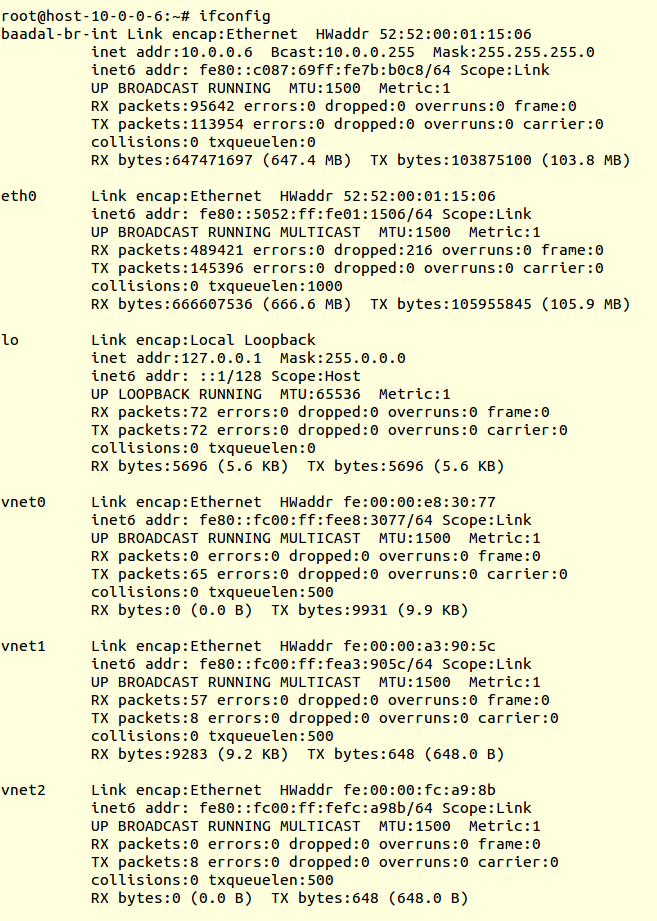
\includegraphics[width=0.9\textwidth]{ifconfig_host6}
\captionof{figure}{Network configuration of host 10.0.0.6}
\end{minipage}

\begin{figure}[h]
\caption{Login inside host 10.0.0.7}
\centering
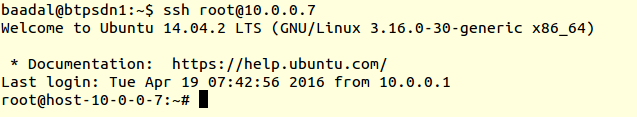
\includegraphics[width=0.9\textwidth]{login_host7}
\end{figure}


\begin{minipage}{\linewidth}

\centering
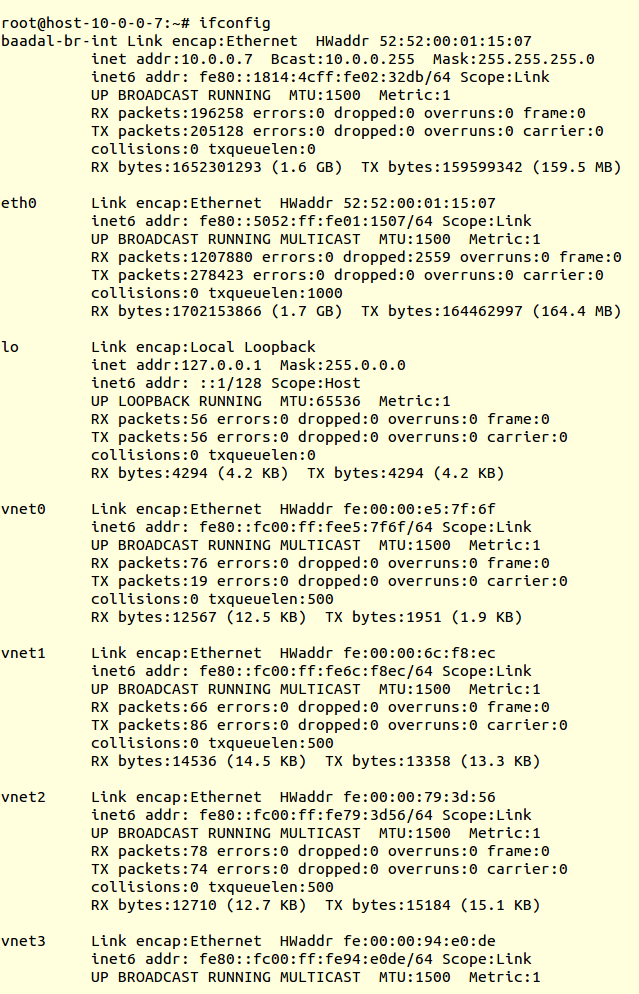
\includegraphics[width=0.9\textwidth]{ifconfig_host7}
\captionof{figure}{Network configuration of host 10.0.0.7}
\end{minipage}

\item \textit{virsh list --all} shows the VMs running inside 10.0.0.6

\begin{minipage}{\linewidth}
\centering
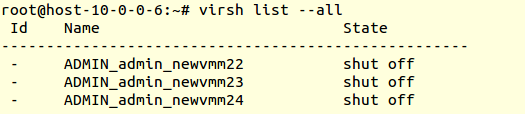
\includegraphics[width=0.9\textwidth]{host6_VMs_shutoff}
\captionof{figure}{VMs shutdown status inside host 10.0.0.6}
\end{minipage}

\begin{minipage}{\linewidth}
\centering
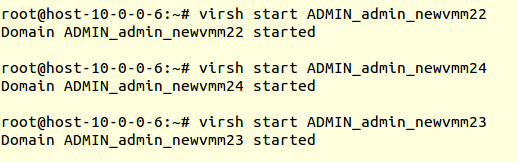
\includegraphics[width=0.9\textwidth]{host6_VMs_start}
\captionof{figure}{Starting VMs inside host 10.0.0.6}
\end{minipage}

\begin{minipage}{\linewidth}
\centering
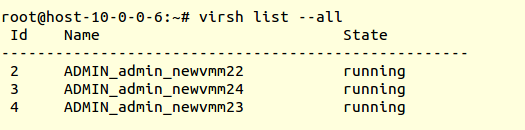
\includegraphics[width=0.9\textwidth]{host6_VMs_running}
\captionof{figure}{Running VMs inside host 10.0.0.6}
\end{minipage}

\item \textit{virsh list --all} shows the VMs running inside 10.0.0.7

\begin{minipage}{\linewidth}
\centering
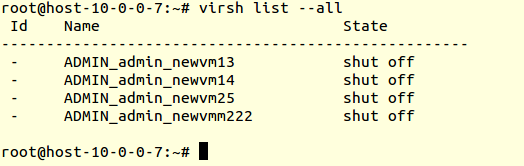
\includegraphics[width=0.9\textwidth]{host7_VMs_shutoff}
\captionof{figure}{VMs shutdown status inside host 10.0.0.7}
\end{minipage}

\begin{minipage}{\linewidth}

\centering
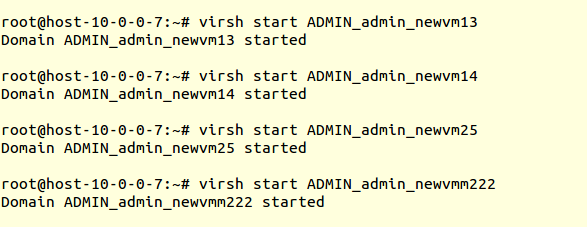
\includegraphics[width=0.9\textwidth]{host7_startinVMs}
\captionof{figure}{Starting VMs inside host 10.0.0.7}
\end{minipage}

\begin{minipage}{\linewidth}
\centering
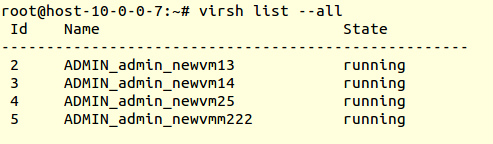
\includegraphics[width=0.9\textwidth]{host7_VMs_running}
\captionof{figure}{Running VMs inside host 10.0.0.7}
\end{minipage}

\item \textit{virt-viewer domain\_name} will open the GUI for the VM whose domain name is specified. Below figure shows for VM \textit{ADMIN\_admin\_newvm25}


\begin{minipage}{\linewidth}
\centering
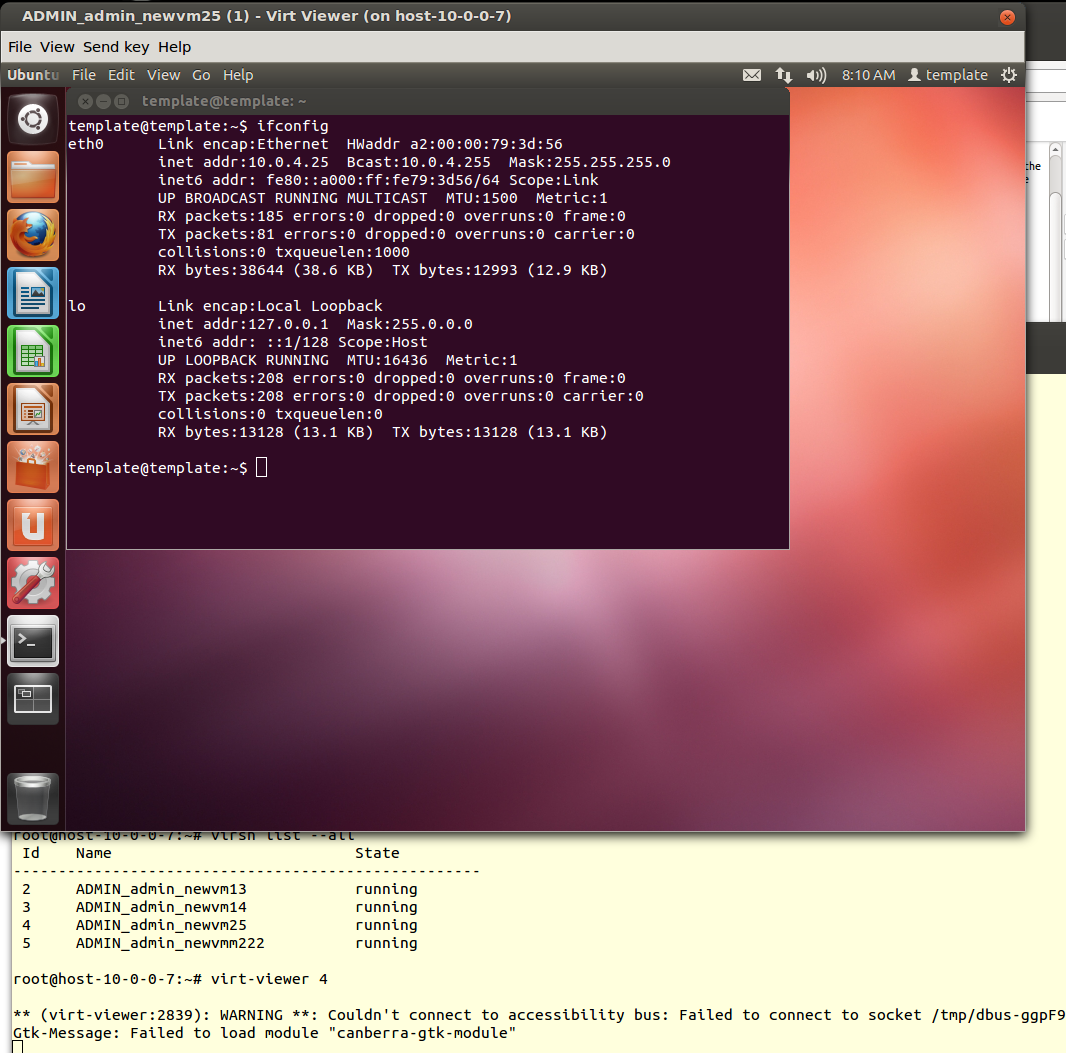
\includegraphics[width=0.9\textwidth]{virt_viewer_host7_ifconfig_425}
\captionof{figure}{Console output for VM 10.0.4.25 after running virt-viewer}
\end{minipage}
\end{enumerate}